\documentclass[11pt]{article}
% Shared preamble for all solution files.
\usepackage[margin=1.1in]{geometry}
\usepackage{enumitem}
\usepackage{tikz}
\usepackage[hidelinks]{hyperref}
\usepackage{amsmath,amssymb,amsthm}
\newcommand{\fa}{\mathfrak a}
\newcommand{\fb}{\mathfrak b}
\newcommand{\fc}{\mathfrak c}
\newcommand{\fp}{\mathfrak p}
\newcommand{\fq}{\mathfrak q}
\newcommand{\fm}{\mathfrak m}
\newcommand{\fn}{\mathfrak n}
\newcommand{\fr}{\mathfrak r}
\newcommand{\Nil}{\mathfrak N}
\newcommand{\Jac}{\mathfrak R}
\newcommand{\rad}{r}
\newcommand{\Spec}{\operatorname{Spec}}
\newcommand{\Max}{\operatorname{Max}}
\newcommand{\Ann}{\operatorname{Ann}}
\newcommand{\Ker}{\operatorname{Ker}}
\newcommand{\Z}{\mathbf Z}
\newcommand{\Q}{\mathbf Q}
\newcommand{\R}{\mathbf R}
\newcommand{\C}{\mathbf C}
\newcommand{\ci}{\mathrm{c}}
\newcommand{\ex}{\mathrm{e}}

\setlength{\parindent}{0pt}
\setlength{\parskip}{0.55em}
% \exercise{label}{statement}  -- followed by the solution text
\newcommand{\exercise}[2]{\par\bigskip\noindent{\large\textbf{Exercise #1}}\par\smallskip
  \begin{quote}\small\textbf{Problem.}\ #2\end{quote}\par}
\newcommand{\pf}{\noindent\textbf{Solution.}\ }

\title{Atiyah--Macdonald, Chapter 1: Rings and Ideals\\[2pt]\large Solutions to the exercises}
\author{}
\date{}
\begin{document}
\maketitle
\noindent\textbf{Conventions.} As in the book, ``ring'' means commutative ring with $1$. $\Nil$ is the nilradical, $\Jac$ the Jacobson radical, $\rad(\fa)$ the radical of an ideal, $X=\Spec A$. For a ring homomorphism $f:A\to B$, $\fa^\ex=Bf(\fa)$ and $\fb^\ci=f^{-1}(\fb)$.

Facts used freely from the text: (1.5) every non-unit lies in a maximal ideal; (1.7) $\Nil$ is an ideal; (1.8) $\Nil=\bigcap$ of all primes; (1.9) $x\in\Jac\iff 1-xy$ is a unit for all $y$; (1.14) $\rad(\fa)=\bigcap_{\fp\supseteq\fa}\fp$.

This chapter covers the three in-text exercises (1.12, 1.13, 1.18) and the 28 end-of-chapter exercises. Exercise 27 contains no assignment as printed (it is exposition leading into Exercise 28); I comment on it at the appropriate place.

%=====================================================================
\section*{In-text exercises}

\exercise{1.12}{Let $\fa,\fb,\fc,\fa_i,\fb_i$ be ideals of a ring $A$, and recall the \emph{ideal quotient} $(\fa:\fb)=\{x\in A: x\fb\subseteq\fa\}$. Prove:
\begin{enumerate}[label=(\roman*),leftmargin=*]
\item $\fa\subseteq(\fa:\fb)$;
\item $(\fa:\fb)\fb\subseteq\fa$;
\item $((\fa:\fb):\fc)=(\fa:\fb\fc)=((\fa:\fc):\fb)$;
\item $\bigl(\bigcap_i\fa_i:\fb\bigr)=\bigcap_i(\fa_i:\fb)$;
\item $\bigl(\fa:\sum_i\fb_i\bigr)=\bigcap_i(\fa:\fb_i)$.
\end{enumerate}}
\pf
(i) If $x\in\fa$ then $x\fb\subseteq\fa$ because $\fa$ is an ideal; so $\fa\subseteq(\fa:\fb)$.

(ii) $(\fa:\fb)\fb$ is generated by products $xy$ with $x\in(\fa:\fb)$, $y\in\fb$; each lies in $\fa$ by definition of $(\fa:\fb)$.

(iii) For $x\in A$:
$x\in((\fa:\fb):\fc)\iff x\fc\subseteq(\fa:\fb)\iff xcb\in\fa$ for all $c\in\fc,b\in\fb$ $\iff x\,(\fb\fc)\subseteq\fa$ (the ideal $\fb\fc$ consists of finite sums of products $bc$, and $\fa$ is closed under sums) $\iff x\in(\fa:\fb\fc)$. The condition ``$xcb\in\fa$ for all $b,c$'' is symmetric in $\fb,\fc$, so also $((\fa:\fc):\fb)=(\fa:\fb\fc)$.

(iv) $x\fb\subseteq\bigcap_i\fa_i\iff x\fb\subseteq\fa_i$ for every $i$.

(v) If $x\fb_i\subseteq\fa$ for all $i$, then $x\sum b_i\subseteq\fa$ (sums of elements of $\fa$). Conversely $\fb_i\subseteq\sum_j\fb_j$. Hence $(\fa:\sum_i\fb_i)=\bigcap_i(\fa:\fb_i)$. \hfill$\square$

\exercise{1.13}{Recall $\rad(\fa)=\{x\in A:x^n\in\fa\text{ for some }n>0\}$. Prove:
\begin{enumerate}[label=(\roman*),leftmargin=*]
\item $\rad(\fa)\supseteq\fa$;
\item $\rad(\rad(\fa))=\rad(\fa)$;
\item $\rad(\fa\fb)=\rad(\fa\cap\fb)=\rad(\fa)\cap\rad(\fb)$;
\item $\rad(\fa)=(1)\iff\fa=(1)$;
\item $\rad(\fa+\fb)=\rad(\rad(\fa)+\rad(\fb))$;
\item if $\fp$ is prime, $\rad(\fp^n)=\fp$ for all $n>0$.
\end{enumerate}}
\pf
(i) $x\in\fa\Rightarrow x^1\in\fa$.

(ii) $\rad(\rad(\fa))\supseteq\rad(\fa)$ by (i). If $x^n\in\rad(\fa)$ then $(x^n)^m\in\fa$ for some $m$, so $x\in\rad(\fa)$.

(iii) Since $\fa\fb\subseteq\fa\cap\fb$ we get $\rad(\fa\fb)\subseteq\rad(\fa\cap\fb)$; since $\fa\cap\fb\subseteq\fa,\fb$ we get $\rad(\fa\cap\fb)\subseteq\rad(\fa)\cap\rad(\fb)$. If $x\in\rad(\fa)\cap\rad(\fb)$, say $x^m\in\fa$, $x^n\in\fb$, then $x^{m+n}\in\fa\fb$, so $x\in\rad(\fa\fb)$. All three coincide.

(iv) $\rad(\fa)=(1)\iff 1\in\rad(\fa)\iff 1^n\in\fa\iff\fa=(1)$.

(v) $\fa\subseteq\rad\fa$, so $\fa+\fb\subseteq\rad\fa+\rad\fb$, hence $\rad(\fa+\fb)\subseteq\rad(\rad\fa+\rad\fb)$. Conversely $\rad\fa,\rad\fb\subseteq\rad(\fa+\fb)$, so $\rad\fa+\rad\fb\subseteq\rad(\fa+\fb)$, and applying $\rad$ and (ii): $\rad(\rad\fa+\rad\fb)\subseteq\rad(\rad(\fa+\fb))=\rad(\fa+\fb)$.

(vi) If $\fp$ is prime, $x^k\in\fp\Rightarrow x\in\fp$, so $\rad(\fp)=\fp$. Then $\fp^n\subseteq\fp$ gives $\rad(\fp^n)\subseteq\fp$; and $x\in\fp\Rightarrow x^n\in\fp^n$ gives $\fp\subseteq\rad(\fp^n)$. \hfill$\square$

\exercise{1.18}{Let $f:A\to B$ be a ring homomorphism, $\fa_1,\fa_2$ ideals of $A$ and $\fb_1,\fb_2$ ideals of $B$. Then
\[
\begin{array}{ll}
(\fa_1+\fa_2)^\ex=\fa_1^\ex+\fa_2^\ex, & (\fb_1+\fb_2)^\ci\supseteq\fb_1^\ci+\fb_2^\ci,\\[2pt]
(\fa_1\cap\fa_2)^\ex\subseteq\fa_1^\ex\cap\fa_2^\ex, & (\fb_1\cap\fb_2)^\ci=\fb_1^\ci\cap\fb_2^\ci,\\[2pt]
(\fa_1\fa_2)^\ex=\fa_1^\ex\fa_2^\ex, & (\fb_1\fb_2)^\ci\supseteq\fb_1^\ci\fb_2^\ci,\\[2pt]
(\fa_1:\fa_2)^\ex\subseteq(\fa_1^\ex:\fa_2^\ex), & (\fb_1:\fb_2)^\ci\subseteq(\fb_1^\ci:\fb_2^\ci),\\[2pt]
\rad(\fa)^\ex\subseteq\rad(\fa^\ex), & \rad(\fb)^\ci=\rad(\fb^\ci).
\end{array}
\]
Deduce that the set $E$ of extended ideals is closed under sum and product, and the set $C$ of contracted ideals is closed under the other three operations ($\cap$, $:$, $\rad$).}
\pf
Let $f:A\to B$.

\emph{Extensions.}
\begin{itemize}[leftmargin=*]
\item $(\fa_1+\fa_2)^\ex=\fa_1^\ex+\fa_2^\ex$: $\supseteq$ since $\fa_i\subseteq\fa_1+\fa_2$; $\subseteq$ since the generators $f(x_1+x_2)=f(x_1)+f(x_2)$ lie in $\fa_1^\ex+\fa_2^\ex$.
\item $(\fa_1\cap\fa_2)^\ex\subseteq\fa_1^\ex\cap\fa_2^\ex$ since $\fa_1\cap\fa_2\subseteq\fa_i$.
\item $(\fa_1\fa_2)^\ex=\fa_1^\ex\fa_2^\ex$: the generators $f(xy)=f(x)f(y)$ of the left side lie in the right; conversely the right side is generated by products $\bigl(\sum b_if(x_i)\bigr)\bigl(\sum b'_jf(x'_j)\bigr)=\sum b_ib'_jf(x_ix'_j)\in(\fa_1\fa_2)^\ex$.
\item $(\fa_1:\fa_2)^\ex\subseteq(\fa_1^\ex:\fa_2^\ex)$: if $x\in(\fa_1:\fa_2)$ then $f(x)f(y)=f(xy)\in f(\fa_1)$ for $y\in\fa_2$, so $f(x)\fa_2^\ex\subseteq\fa_1^\ex$, i.e.\ $f(x)\in(\fa_1^\ex:\fa_2^\ex)$; the latter is an ideal, hence contains the ideal generated by these $f(x)$.
\item $\rad(\fa)^\ex\subseteq\rad(\fa^\ex)$: if $x^n\in\fa$ then $f(x)^n\in\fa^\ex$, so $f(x)\in\rad(\fa^\ex)$, an ideal.
\end{itemize}

\emph{Contractions.} Preimages respect all inclusions, so:
\begin{itemize}[leftmargin=*]
\item $(\fb_1+\fb_2)^\ci\supseteq\fb_1^\ci+\fb_2^\ci$ (monotonicity).
\item $(\fb_1\cap\fb_2)^\ci=\fb_1^\ci\cap\fb_2^\ci$ (preimage of an intersection).
\item $(\fb_1\fb_2)^\ci\supseteq\fb_1^\ci\fb_2^\ci$: for $x\in\fb_1^\ci,y\in\fb_2^\ci$, $f(xy)=f(x)f(y)\in\fb_1\fb_2$.
\item $(\fb_1:\fb_2)^\ci\subseteq(\fb_1^\ci:\fb_2^\ci)$: if $f(x)\fb_2\subseteq\fb_1$ and $y\in\fb_2^\ci$ then $f(xy)=f(x)f(y)\in\fb_1$, so $xy\in\fb_1^\ci$.
\item $\rad(\fb)^\ci=\rad(\fb^\ci)$: $x\in\rad(\fb)^\ci\iff f(x)^n\in\fb$ some $n\iff x^n\in\fb^\ci$ some $n$.
\end{itemize}

\emph{$E$ is closed under $+,\cdot$; $C$ is closed under $\cap,:,\rad$.} Recall $C=\{\fa:\fa=\fa^{\ex\ci}\}$, $E=\{\fb:\fb=\fb^{\ci\ex}\}$.

If $\fb_1,\fb_2\in E$, then $\fb_1+\fb_2=\fb_1^{\ci\ex}+\fb_2^{\ci\ex}=(\fb_1^\ci+\fb_2^\ci)^\ex\in E$ and $\fb_1\fb_2=(\fb_1^\ci)^\ex(\fb_2^\ci)^\ex=(\fb_1^\ci\fb_2^\ci)^\ex\in E$ (extended ideals are in $E$ by 1.17).

If $\fa_1,\fa_2,\fa\in C$ then, using the displayed inclusions and $\fa=\fa^{\ex\ci}$:
\begin{align*}
(\fa_1\cap\fa_2)^{\ex\ci}&\subseteq(\fa_1^\ex\cap\fa_2^\ex)^\ci=\fa_1^{\ex\ci}\cap\fa_2^{\ex\ci}=\fa_1\cap\fa_2,\\
(\fa_1:\fa_2)^{\ex\ci}&\subseteq(\fa_1^\ex:\fa_2^\ex)^\ci\subseteq(\fa_1^{\ex\ci}:\fa_2^{\ex\ci})=(\fa_1:\fa_2),\\
\rad(\fa)^{\ex\ci}&\subseteq\rad(\fa^\ex)^\ci=\rad(\fa^{\ex\ci})=\rad(\fa).
\end{align*}
The reverse inclusions hold always (1.17(i)), so these ideals lie in $C$. \hfill$\square$

%=====================================================================
\section*{End-of-chapter exercises}

%---------------------------------------------------------------- 1
\exercise{1}{Let $x$ be a nilpotent element of a ring $A$. Show that $1+x$ is a unit of $A$. Deduce that the sum of a nilpotent element and a unit is a unit.}
\pf
Let $x^n=0$. Then $(1+x)\bigl(1-x+x^2-\cdots+(-1)^{n-1}x^{n-1}\bigr)=1+(-1)^{n-1}x^n=1$.
If $u$ is a unit and $x$ nilpotent, then $u^{-1}x$ is nilpotent (commutativity) so $u+x=u(1+u^{-1}x)$ is a product of units. \hfill$\square$

%---------------------------------------------------------------- 2
\exercise{2}{Let $A$ be a ring and let $A[x]$ be the ring of polynomials in an indeterminate $x$, with coefficients in $A$. Let $f=a_0+a_1x+\cdots+a_nx^n\in A[x]$. Prove that
\begin{enumerate}[label=(\roman*),leftmargin=*]
\item $f$ is a unit in $A[x]\iff a_0$ is a unit in $A$ and $a_1,\dots,a_n$ are nilpotent. [If $b_0+b_1x+\cdots+b_mx^m$ is the inverse of $f$, prove by induction on $r$ that $a_n^{r+1}b_{m-r}=0$. Hence show that $a_n$ is nilpotent, and then use Ex.~1.]
\item $f$ is nilpotent $\iff a_0,a_1,\dots,a_n$ are nilpotent.
\item $f$ is a zero-divisor $\iff$ there exists $a\ne0$ in $A$ such that $af=0$. [Choose a polynomial $g=b_0+b_1x+\cdots+b_mx^m$ of least degree $m$ such that $fg=0$. Then $a_nb_m=0$, hence $a_ng=0$ (because $a_ng$ annihilates $f$ and has degree $<m$). Now show by induction that $a_{n-r}g=0$ $(0\le r\le n)$.]
\item $f$ is said to be \emph{primitive} if $(a_0,a_1,\dots,a_n)=(1)$. Prove that if $f,g\in A[x]$, then $fg$ is primitive $\iff f$ and $g$ are primitive.
\end{enumerate}}
\pf
Let $f=a_0+a_1x+\dots+a_nx^n$.

\textbf{(i) $f$ is a unit $\iff a_0$ is a unit and $a_1,\dots,a_n$ are nilpotent.}

($\Leftarrow$) Each $a_ix^i$ ($i\ge1$) is nilpotent, and nilpotents form an ideal (1.7), so $f-a_0$ is nilpotent; apply Exercise 1.

($\Rightarrow$) Let $fg=1$, $g=b_0+\dots+b_mx^m$. Then $a_0b_0=1$, so $a_0$ is a unit. We prove by induction on $r$ ($0\le r\le m$) that
\[
S(r):\quad a_n^{\,r+1}b_{m-r}=0 .
\]
Assume $n\ge1$ (else nothing to prove). $S(0)$: the coefficient of $x^{n+m}$ in $fg$ is $a_nb_m=0$. For $r\ge1$ assume $S(0),\dots,S(r-1)$. The coefficient of $x^{n+m-r}$ ($\ge n\ge 1$) in $fg$ is zero:
$\sum_{k=0}^{r}a_{n-k}b_{m-r+k}=0$ (with $a_i=0$ for $i<0$). Multiply by $a_n^{r}$:
\[
a_n^{r+1}b_{m-r}+\sum_{k=1}^{r}a_{n-k}\,a_n^{k-1}\bigl(a_n^{\,r-k+1}b_{m-(r-k)}\bigr)=0,
\]
and each bracket vanishes by $S(r-k)$. So $S(r)$ holds. Taking $r=m$: $a_n^{m+1}b_0=0$, and $b_0$ is a unit, so $a_n$ is nilpotent.

Now $a_nx^n$ is nilpotent, so $f-a_nx^n$ is a unit (unit minus nilpotent, Ex.~1) of degree $<n$, with the same $a_0,\dots,a_{n-1}$. By induction on $n$ (the case $n=0$ is trivial) $a_1,\dots,a_{n-1}$ are nilpotent.

\textbf{(ii) $f$ nilpotent $\iff$ all $a_i$ nilpotent.} ($\Leftarrow$) as in (i): $\Nil(A[x])$ is an ideal containing each $a_ix^i$. ($\Rightarrow$) Let $\fp$ be a prime of $A$. Then $\fp A[x]$ (polynomials with all coefficients in $\fp$) is prime in $A[x]$, because $A[x]/\fp A[x]\cong(A/\fp)[x]$ is a domain. A nilpotent $f$ lies in every prime of $A[x]$ (1.8), so all $a_i\in\fp$. Hence $a_i\in\bigcap\fp=\Nil(A)$.

\textbf{(iii) $f$ is a zero-divisor $\iff\exists a\ne0$ with $af=0$.} ($\Leftarrow$) clear. ($\Rightarrow$) Choose $g=b_0+\dots+b_mx^m\ne0$ with $fg=0$ and $m$ minimal. Then $a_nb_m=0$, so $a_ng$ has degree $<m$ and $f(a_ng)=0$; minimality gives $a_ng=0$. We show by induction on $r=0,\dots,n$ that $a_{n-r}g=0$. Suppose $a_{n-s}g=0$ for $s<r$. The coefficient of $x^{n+m-r}$ in $fg$ is $\sum_{s=0}^{r}a_{n-s}b_{m-r+s}=0$; the terms with $s<r$ vanish, so $a_{n-r}b_m=0$. Then $a_{n-r}g$ has degree $<m$ and is killed by $f$, so $a_{n-r}g=0$. Hence $a_ig=0$ for all $i$; in particular $a:=b_m\neq0$ satisfies $a_ib_m=0$ for all $i$, i.e.\ $b_mf=0$.

\textbf{(iv) For $f,g\in A[x]$: $fg$ primitive $\iff f$ and $g$ primitive.} Let $c(f)$ be the ideal generated by the coefficients. Each coefficient of $fg$ is a sum of products $a_ib_j$, so $c(fg)\subseteq c(f)\cap c(g)$; hence $fg$ primitive forces $c(f)=c(g)=(1)$. Conversely suppose $f,g$ primitive but $c(fg)\ne(1)$. Then $c(fg)\subseteq\fm$ for a maximal ideal $\fm$, so $fg\in\fm A[x]$, which is prime ($A[x]/\fm A[x]=(A/\fm)[x]$ is a domain). Thus $f\in\fm A[x]$ or $g\in\fm A[x]$, i.e.\ $c(f)\subseteq\fm$ or $c(g)\subseteq\fm$, contradicting primitivity. \hfill$\square$

%---------------------------------------------------------------- 3
\exercise{3}{Generalize the results of Exercise 2 to a polynomial ring $A[x_1,\dots,x_r]$ in several indeterminates.}
\pf
Write $A_r=A[x_1,\dots,x_r]$. The statements are:
\begin{enumerate}[label=(\roman*),leftmargin=*]
\item $f\in A_r$ is a unit $\iff$ its constant term is a unit of $A$ and all its other coefficients are nilpotent;
\item $f$ is nilpotent $\iff$ all its coefficients are nilpotent;
\item $f$ is a zero-divisor $\iff\exists a\in A$, $a\ne0$, $af=0$;
\item $f,g$ are primitive (coefficients generate $(1)$) $\iff fg$ is primitive.
\end{enumerate}
(i), (ii): induct on $r$, using $A_r=A_{r-1}[x_r]$. Write $f=\sum_kf_kx_r^k$ with $f_k\in A_{r-1}$. By Ex.~2, $f$ is a unit iff $f_0$ is a unit and $f_k$ ($k\ge1$) are nilpotent in $A_{r-1}$; by induction this says: the constant term of $f_0$ (= constant term of $f$) is a unit and all other coefficients of $f_0$ are nilpotent, and all coefficients of the $f_k$, $k\ge1$, are nilpotent. Same for (ii).

(iii) ($\Leftarrow$) clear. ($\Rightarrow$) (Kronecker substitution.) Let $fg=0$, $g\neq0$. Choose $d$ larger than every exponent of every variable occurring in $f$ or $g$, and let $\kappa:A_r\to A[t]$ be the ring homomorphism $x_i\mapsto t^{d^{\,i-1}}$. By uniqueness of base-$d$ expansions, distinct monomials with all exponents $<d$ go to distinct powers of $t$; so $\kappa$ is injective on the polynomials all of whose exponents are $<d$ (this includes $f,g$, and $af$ for $a\in A$). Thus $\kappa(g)\ne0$ and $\kappa(f)\kappa(g)=0$, so $\kappa(f)$ is a zero-divisor of $A[t]$, and by Ex.~2(iii) there is $a\ne0$ with $a\kappa(f)=\kappa(af)=0$; injectivity gives $af=0$.

(iv) Identical to Ex.~2(iv): $c(fg)\subseteq c(f)\cap c(g)$ for $\Rightarrow$, and for $\Leftarrow$ use $\fm A_r$ prime since $A_r/\fm A_r\cong(A/\fm)[x_1,\dots,x_r]$ is a domain. \hfill$\square$

%---------------------------------------------------------------- 4
\exercise{4}{In the ring $A[x]$, the Jacobson radical is equal to the nilradical.}
\pf
Always $\Nil\subseteq\Jac$ (nilpotent elements lie in every prime, in particular every maximal ideal). Let $f=\sum a_ix^i\in\Jac(A[x])$. By 1.9 (with $y=x$), $1-xf=1-a_0x-a_1x^2-\cdots$ is a unit. By Ex.~2(i), all of $-a_0,-a_1,\dots$ are nilpotent. By Ex.~2(ii), $f$ is nilpotent. \hfill$\square$

%---------------------------------------------------------------- 5
\exercise{5}{Let $A$ be a ring and let $A[[x]]$ be the ring of formal power series $f=\sum_{n=0}^\infty a_nx^n$ with coefficients in $A$. Show that
\begin{enumerate}[label=(\roman*),leftmargin=*]
\item $f$ is a unit in $A[[x]]\iff a_0$ is a unit in $A$.
\item If $f$ is nilpotent, then $a_n$ is nilpotent for all $n\ge0$. Is the converse true? (See Chapter 7, Exercise 2.)
\item $f$ belongs to the Jacobson radical of $A[[x]]\iff a_0$ belongs to the Jacobson radical of $A$.
\item The contraction of a maximal ideal $\fm$ of $A[[x]]$ is a maximal ideal of $A$, and $\fm$ is generated by $\fm^\ci$ and $x$.
\item Every prime ideal of $A$ is the contraction of a prime ideal of $A[[x]]$.
\end{enumerate}}
\pf
Let $f=\sum a_nx^n$.

\textbf{(i)} If $fg=1$ then $a_0b_0=1$. Conversely if $a_0$ is a unit, define $b_0=a_0^{-1}$ and recursively $b_n=-a_0^{-1}\sum_{i=1}^na_ib_{n-i}$; then $g=\sum b_nx^n$ satisfies $fg=1$.

\textbf{(ii)} Let $f^N=0$ and let $\fp$ be a prime of $A$. Reducing coefficients gives a ring homomorphism $A[[x]]\to(A/\fp)[[x]]$, and $(A/\fp)[[x]]$ is a domain (the product of the lowest-order terms $\bar a_rx^r,\bar b_sx^s$ of two nonzero series has coefficient $\bar a_r\bar b_s\ne0$ at $x^{r+s}$). So $\bar f=0$, i.e.\ all $a_n\in\fp$. Hence $a_n\in\bigcap\fp=\Nil(A)$.

\emph{The converse is false.} Let $k$ be a field and $A=k[t_1,t_2,\dots]/(t_1,t_2^2,t_3^3,\dots)$. Each $t_n$ is nilpotent ($t_n^n=0$). Put $f=\sum_{n\ge1}t_nx^n$. Suppose $f^N=0$ and take $n>N$. The coefficient of $x^{nN}$ in $f^N$ is $\sum t_{i_1}\cdots t_{i_N}$ over ordered tuples with $i_1+\dots+i_N=nN$. $A$ has the $k$-basis of monomials $\prod t_i^{e_i}$ with $e_i<i$; the monomial $t_n^N$ (note $N<n$) is such a basis element, and it arises from only one tuple, $(n,\dots,n)$, while every other tuple gives a different monomial (or $0$). So this coefficient is nonzero, contradicting $f^N=0$. So $f$ is not nilpotent although all its coefficients are.

\textbf{(iii)} By 1.9, $f\in\Jac(A[[x]])\iff1-fg$ is a unit for all $g\in A[[x]]$ $\iff$ (by (i)) $1-a_0b_0$ is a unit in $A$ for all $g$, i.e.\ for all $b_0\in A$ (constants are allowed as $g$) $\iff a_0\in\Jac(A)$.

\textbf{(iv)} Let $\fm$ be maximal in $A[[x]]$. First $x\in\fm$: otherwise $\fm+(x)=(1)$, so $1=h+gx$ with $h\in\fm$, and $h=1-gx$ is a unit by (i), absurd. Let $\varepsilon:A[[x]]\to A$, $f\mapsto a_0$, with kernel $(x)$; it is surjective. Since $(x)\subseteq\fm$, $\fm=\varepsilon^{-1}(\fm')$ with $\fm'=\varepsilon(\fm)$ maximal in $A$ (Prop.~1.1: $\fm/(x)$ is maximal in $A[[x]]/(x)\cong A$). Constants satisfy $\varepsilon(a)=a$, so $\fm^\ci=\fm\cap A=\fm'$ is maximal in $A$. Finally every $f\in\fm$ is $a_0+xh$ with $a_0\in\fm'=\fm^\ci$, so $\fm=\fm^\ex+(x)$, i.e.\ $\fm$ is generated by $\fm^\ci$ and $x$; the reverse inclusion is obvious.

\textbf{(v)} For a prime $\fp$ of $A$ let $P=\varepsilon^{-1}(\fp)=\{f:a_0\in\fp\}$. Then $A[[x]]/P\cong A/\fp$ is a domain, so $P$ is prime, and $P^\ci=P\cap A=\fp$. \hfill$\square$

%---------------------------------------------------------------- 6
\exercise{6}{A ring $A$ is such that every ideal not contained in the nilradical contains a non-zero idempotent (that is, an element $e$ such that $e^2=e\ne0$). Prove that the nilradical and Jacobson radical of $A$ are equal.}
\pf
$\Nil\subseteq\Jac$ always. Suppose $\Jac\not\subseteq\Nil$. Then the ideal $\Jac$ contains an idempotent $e\ne0$. By 1.9, $1-e=1-e\cdot1$ is a unit. But $e(1-e)=e-e^2=0$, so $e=0$, contradiction. Hence $\Jac\subseteq\Nil$. \hfill$\square$

%---------------------------------------------------------------- 7
\exercise{7}{Let $A$ be a ring in which every element $x$ satisfies $x^n=x$ for some $n>1$ (depending on $x$). Show that every prime ideal in $A$ is maximal.}
\pf
Let $\fp$ be prime and $D=A/\fp$, a domain in which every element also satisfies $\bar x^n=\bar x$, some $n>1$. If $\bar x\ne0$ then $\bar x(\bar x^{n-1}-1)=0$ forces $\bar x^{n-1}=1$, i.e.\ $\bar x\cdot\bar x^{n-2}=1$; so $\bar x$ is a unit. Thus $D$ is a field and $\fp$ is maximal. \hfill$\square$

%---------------------------------------------------------------- 8
\exercise{8}{Let $A$ be a ring $\ne0$. Show that the set of prime ideals of $A$ has minimal elements with respect to inclusion.}
\pf
Let $\Sigma$ be the set of primes, ordered by reverse inclusion; it is nonempty since $A\ne0$ has a maximal ideal. We show every chain $(\fp_\alpha)$ has an upper bound (i.e.\ the intersection $\fp=\bigcap\fp_\alpha$ is prime). $1\notin\fp$. Suppose $xy\in\fp$ and $x\notin\fp$, say $x\notin\fp_\beta$. Let $\alpha$ be arbitrary. If $\fp_\alpha\subseteq\fp_\beta$, then $x\notin\fp_\alpha$ and $xy\in\fp_\alpha$ give $y\in\fp_\alpha$. If $\fp_\beta\subseteq\fp_\alpha$, then $xy\in\fp_\beta$ and $x\notin\fp_\beta$ give $y\in\fp_\beta\subseteq\fp_\alpha$. So $y\in\fp$. By Zorn, $\Sigma$ has a maximal element for reverse inclusion, i.e.\ a minimal prime ideal. (Indeed every prime contains a minimal prime.) \hfill$\square$

%---------------------------------------------------------------- 9
\exercise{9}{Let $\fa$ be an ideal $\ne(1)$ in a ring $A$. Show that $\fa=\rad(\fa)\iff\fa$ is an intersection of prime ideals.}
\pf
($\Rightarrow$) $\rad(\fa)=\bigcap_{\fp\supseteq\fa}\fp$ by 1.14. ($\Leftarrow$) If $\fa=\bigcap_i\fp_i$ then $\rad(\fa)\subseteq\rad(\fp_i)=\fp_i$ for each $i$, so $\rad(\fa)\subseteq\fa$; and $\fa\subseteq\rad(\fa)$ always. \hfill$\square$

%---------------------------------------------------------------- 10
\exercise{10}{Let $A$ be a ring, $\Nil$ its nilradical. Show that the following are equivalent:
\begin{enumerate}[label=(\roman*),leftmargin=*]
\item $A$ has exactly one prime ideal;
\item every element of $A$ is either a unit or nilpotent;
\item $A/\Nil$ is a field.
\end{enumerate}}
\pf
(Assume $A\ne0$.)
(i)$\Rightarrow$(ii): If $\fp$ is the only prime then $\Nil=\fp$ (1.8). A non-unit lies in a maximal ideal, which is prime, hence equals $\fp=\Nil$, so the non-unit is nilpotent.
(ii)$\Rightarrow$(iii): $A/\Nil\ne0$. If $\bar x\ne0$ then $x$ is not nilpotent, hence a unit, hence $\bar x$ is a unit.
(iii)$\Rightarrow$(i): $\Nil$ is maximal, hence prime. Every prime contains $\Nil=\bigcap\fp$, hence equals the maximal ideal $\Nil$. \hfill$\square$

%---------------------------------------------------------------- 11
\exercise{11}{A ring $A$ is \emph{Boolean} if $x^2=x$ for all $x\in A$. In a Boolean ring $A$, show that
\begin{enumerate}[label=(\roman*),leftmargin=*]
\item $2x=0$ for all $x\in A$;
\item every prime ideal $\fp$ is maximal, and $A/\fp$ is a field with two elements;
\item every finitely generated ideal in $A$ is principal.
\end{enumerate}}
\pf
(i) $2x=(x+x)^2=\ldots$: $(2x)^2=4x^2=4x$ and $(2x)^2=2x$, so $4x=2x$, hence $2x=0$.

(ii) Let $\fp$ be prime. In the domain $A/\fp$ every $\bar x$ satisfies $\bar x(\bar x-1)=0$, so $\bar x\in\{0,1\}$. Thus $A/\fp=\{0,1\}\cong\mathbf F_2$ is a field and $\fp$ is maximal.

(iii) For $x,y\in A$ put $z=x+y+xy\in(x,y)$. Then $xz=x+xy+xy=x+2xy=x$ and likewise $yz=y$, so $(x,y)\subseteq(z)\subseteq(x,y)$. By induction on the number of generators every finitely generated ideal is principal. \hfill$\square$

%---------------------------------------------------------------- 12
\exercise{12}{A local ring contains no idempotent $\ne0,1$.}
\pf
Let $\fm$ be the maximal ideal and $e^2=e$, so $e(1-e)=0$. Not both $e,1-e$ lie in $\fm$ (else $1\in\fm$). If $e\notin\fm$, $e$ is a unit (all elements outside $\fm$ are, by 1.6), so $1-e=0$, $e=1$. If $1-e\notin\fm$, then $1-e$ is a unit and $e=0$. \hfill$\square$

%---------------------------------------------------------------- 13
\exercise{13}{(\emph{Construction of an algebraic closure of a field}, E.~Artin.) Let $K$ be a field and let $\Sigma$ be the set of all irreducible monic polynomials $f$ in one indeterminate with coefficients in $K$. Let $A$ be the polynomial ring over $K$ generated by indeterminates $x_f$, one for each $f\in\Sigma$. Let $\fa$ be the ideal of $A$ generated by the polynomials $f(x_f)$ for all $f\in\Sigma$. Show that $\fa\ne(1)$.

Let $\fm$ be a maximal ideal of $A$ containing $\fa$, and let $K_1=A/\fm$. Then $K_1$ is an extension field of $K$ in which each $f\in\Sigma$ has a root. Repeat the construction with $K_1$ in place of $K$, obtaining a field $K_2$, and so on. Let $L=\bigcup_{n=1}^\infty K_n$. Then $L$ is a field in which each $f\in\Sigma$ splits completely into linear factors. Let $\bar K$ be the set of all elements of $L$ which are algebraic over $K$. Then $\bar K$ is an algebraic closure of $K$.}
\pf
Let $A=K[x_f:f\in\Sigma]$ and $\fa=\bigl(f(x_f):f\in\Sigma\bigr)$.

\textbf{$\fa\ne(1)$.} Suppose $1=\sum_{i=1}^ng_if_i(x_{f_i})$ with $g_i\in A$ and $f_1,\dots,f_n\in\Sigma$ distinct. Let $F$ be a finite extension field of $K$ in which each $f_i$ has a root $\alpha_i$ (adjoin roots one at a time: $K[t]/(\text{irreducible factor})$). The $K$-algebra homomorphism $A\to F$ with $x_{f_i}\mapsto\alpha_i$ ($i\le n$) and all other $x_f\mapsto0$ sends the relation to $1=0$, absurd.

\textbf{The tower.} Take a maximal ideal $\fm\supseteq\fa$ (1.4) and $K_1=A/\fm$. Since $K$ is a field, $K\to K_1$ is injective; the image of $x_f$ is a root of $f$ in $K_1$. Repeat with $K_1$ in place of $K$ to get $K_2$, etc., and put $L=\bigcup_nK_n$, a field (union of a chain of fields).

\textbf{Claim: every non-constant $h\in K_n[t]$ has a root in $K_{n+1}$.} Let $g$ be a monic irreducible factor of $h$ over $K_n$; $g$ has a root in $K_{n+1}$ by construction, and it is a root of $h$.
Hence if $f\in K[t]$ has degree $d$, it has a root in $K_1$, so $f=(t-\alpha_1)f_1$ in $K_1[t]$; $f_1$ has a root in $K_2$; etc. After $d$ steps $f$ splits into linear factors in $K_d[t]\subseteq L[t]$. So every $f\in\Sigma$ splits completely in $L$.

\textbf{$\bar K$ is an algebraic closure.} Let $\bar K\subseteq L$ be the set of elements algebraic over $K$; it is a subfield (standard: $K(\alpha,\beta)$ is finite over $K$). Every $f\in K[t]$ splits into linear factors in $L[t]$, and its roots there are algebraic over $K$, so $f$ splits completely in $\bar K[t]$. Now let $h\in\bar K[t]$ be irreducible and let $\beta$ be a root of $h$ in the extension field $E=\bar K[t]/(h)$. Then $\beta$ is algebraic over $\bar K$, which is algebraic over $K$, so $\beta$ is algebraic over $K$ (finite towers), i.e.\ a root of some $f\in K[t]$, $f\ne0$. As $f=\prod(t-\gamma_i)$ with $\gamma_i\in\bar K$, $\beta=\gamma_i\in\bar K$. So $h$ has a root in $\bar K$, hence is linear. Thus $\bar K$ is algebraically closed and algebraic over $K$, i.e.\ an algebraic closure of $K$. \hfill$\square$

%---------------------------------------------------------------- 14
\exercise{14}{In a ring $A$, let $\Sigma$ be the set of all ideals in which every element is a zero-divisor. Show that the set $\Sigma$ has maximal elements and that every maximal element of $\Sigma$ is a prime ideal. Hence the set of zero-divisors in $A$ is a union of prime ideals.}
\pf
(Assume $A\ne0$.) $\Sigma\ni(0)$ is nonempty. The union of a chain in $\Sigma$ is an ideal all of whose elements are zero-divisors; so Zorn gives maximal elements of $\Sigma$, and more precisely, for each ideal $\fa\in\Sigma$, a maximal element of $\Sigma$ containing it.

Let $\fp$ be maximal in $\Sigma$. $\fp\ne(1)$ since $1$ is not a zero-divisor. Suppose $xy\in\fp$ with $x,y\notin\fp$. By maximality $\fp+(x)\notin\Sigma$ and $\fp+(y)\notin\Sigma$, so there exist non-zero-divisors $u=p_1+ax$ and $v=p_2+by$ ($p_i\in\fp$). Then $uv=p_1p_2+p_1by+p_2ax+ab\,xy\in\fp$, and $uv$ is a non-zero-divisor (a product of two non-zero-divisors), contradicting $\fp\in\Sigma$. So $\fp$ is prime.

Finally let $D$ be the set of zero-divisors. Each maximal element of $\Sigma$ is a prime contained in $D$. Conversely, if $x\in D$ with $xy=0$, $y\ne0$, then every $ax$ is a zero-divisor ($axy=0$), so $(x)\in\Sigma$ and $(x)$ lies in a maximal element of $\Sigma$, a prime. Therefore $D$ is the union of these primes. \hfill$\square$

%---------------------------------------------------------------- 15
\exercise{15}{(\emph{The prime spectrum of a ring.}) Let $A$ be a ring and let $X$ be the set of all prime ideals of $A$. For each subset $E$ of $A$, let $V(E)$ denote the set of all prime ideals of $A$ which contain $E$. Prove that
\begin{enumerate}[label=(\roman*),leftmargin=*]
\item if $\fa$ is the ideal generated by $E$, then $V(E)=V(\fa)=V(\rad(\fa))$;
\item $V(0)=X$, $V(1)=\emptyset$;
\item if $(E_i)_{i\in I}$ is any family of subsets of $A$, then $V\bigl(\bigcup_{i\in I}E_i\bigr)=\bigcap_{i\in I}V(E_i)$;
\item $V(\fa\cap\fb)=V(\fa\fb)=V(\fa)\cup V(\fb)$ for any ideals $\fa,\fb$ of $A$.
\end{enumerate}
These results show that the sets $V(E)$ satisfy the axioms for closed sets in a topological space. The resulting topology is called the \emph{Zariski topology}. The topological space $X$ is called the \emph{prime spectrum} of $A$, and is written $\Spec(A)$.}
\pf
\textbf{(i)} A prime contains $E\iff$ it contains the ideal $\fa=(E)$ generated by $E$. A prime $\fp\supseteq\fa$ contains $\rad(\fa)$ (if $x^n\in\fa\subseteq\fp$ then $x\in\fp$); conversely $\fp\supseteq\rad(\fa)\supseteq\fa$. So $V(E)=V(\fa)=V(\rad\fa)$.

\textbf{(ii)} Every prime contains $0$: $V(0)=X$. No prime contains $1$: $V(1)=\emptyset$.

\textbf{(iii)} $\fp\supseteq\bigcup E_i\iff\fp\supseteq E_i$ for all $i$. So $V(\bigcup E_i)=\bigcap V(E_i)$.

\textbf{(iv)} $\fa\fb\subseteq\fa\cap\fb\subseteq\fa,\fb$ gives $V(\fa)\cup V(\fb)\subseteq V(\fa\cap\fb)\subseteq V(\fa\fb)$. If $\fp\supseteq\fa\fb$ and $\fp\not\supseteq\fa$, pick $x\in\fa\setminus\fp$; for each $y\in\fb$, $xy\in\fp$, so $y\in\fp$, i.e.\ $\fp\supseteq\fb$. So $V(\fa\fb)\subseteq V(\fa)\cup V(\fb)$. All four sets agree. \hfill$\square$

%---------------------------------------------------------------- 16
\exercise{16}{Draw pictures of $\Spec(\Z)$, $\Spec(\R)$, $\Spec(\C[x])$, $\Spec(\R[x])$, $\Spec(\Z[x])$.}
\pf
In each picture a line from a point $\fq$ upward to $\fp$ means $\fq\subset\fp$ (so $\fp$ lies in the closure of $\fq$: $\fq$ is ``more generic''). Closed sets are $V(E)$; closed points are maximal ideals.

\begin{center}
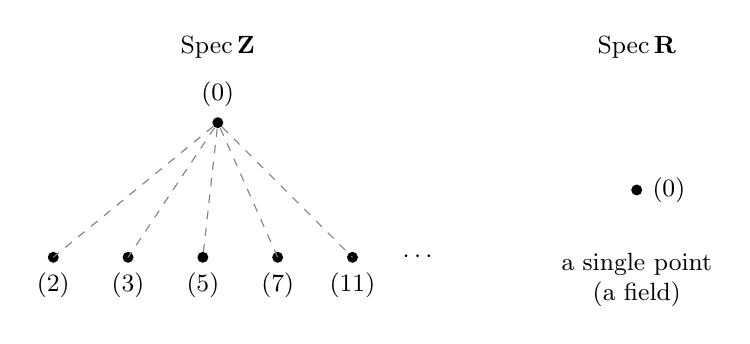
\begin{tikzpicture}[scale=0.95,every node/.style={font=\small},dot/.style={circle,fill,inner sep=1.4pt}]
% Spec Z
\begin{scope}
\node at (2.6,3.6) {\textbf{$\Spec\Z$}};
\node[dot,label=above:{$(0)$}] (g) at (2.6,2.6) {};
\foreach \x/\l in {0.4/2,1.4/3,2.4/5,3.4/7,4.4/11}{
  \node[dot,label=below:{$(\l)$}] at (\x,0.8) {};
  \draw[dashed,gray] (g) -- (\x,0.8);}
\node at (5.3,0.8) {$\cdots$};
\end{scope}
% Spec R
\begin{scope}[xshift=7.2cm]
\node at (1,3.6) {\textbf{$\Spec\R$}};
\node[dot,label=right:{$(0)$}] at (1,1.7) {};
\node[align=center] at (1,0.5) {a single point\\(a field)};
\end{scope}
\end{tikzpicture}
\end{center}

\emph{$\Spec\Z$:} points $(0)$ and $(p)$, $p$ prime. $V(n)=\{(p):p\mid n\}$ for $n\neq0$ is finite, so the proper closed sets are the finite sets of closed points; $(0)$ is dense (the generic point).
\emph{$\Spec\R$:} one point $(0)$.

\begin{center}
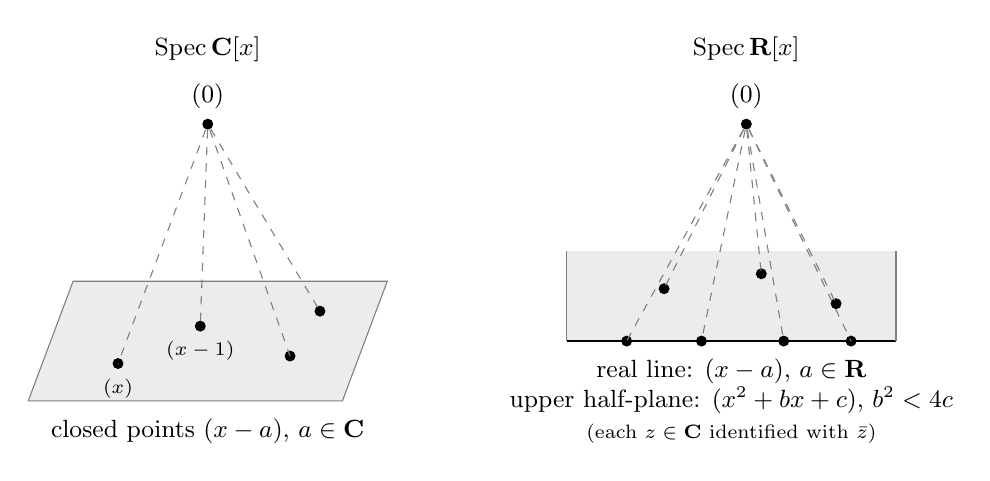
\begin{tikzpicture}[scale=0.95,every node/.style={font=\small},dot/.style={circle,fill,inner sep=1.4pt}]
% Spec C[x]
\begin{scope}
\node at (2.4,4.7) {\textbf{$\Spec\C[x]$}};
\node[dot,label=above:{$(0)$}] (g) at (2.4,3.7) {};
\fill[gray!15] (0,0) -- (4.2,0) -- (4.8,1.6) -- (0.6,1.6) -- cycle;
\draw[gray] (0,0) -- (4.2,0) -- (4.8,1.6) -- (0.6,1.6) -- cycle;
\foreach \x/\y/\l in {1.2/0.5/0,2.3/1.0/1,3.5/0.6/i,3.9/1.2/{2+i}}{
  \node[dot] at (\x,\y) {};
  \draw[dashed,gray] (g) -- (\x,\y);}
\node[below=2pt] at (1.2,0.5) {\scriptsize $(x)$};
\node[below=2pt] at (2.3,1.0) {\scriptsize $(x-1)$};
\node at (2.4,-0.4) {closed points $(x-a)$, $a\in\C$};
\end{scope}
% Spec R[x]
\begin{scope}[xshift=7.2cm]
\node at (2.4,4.7) {\textbf{$\Spec\R[x]$}};
\node[dot,label=above:{$(0)$}] (g) at (2.4,3.7) {};
\fill[gray!15] (0,0.8) rectangle (4.4,2.0);
\draw[thick] (0,0.8) -- (4.4,0.8);
\draw[gray] (0,2.0) -- (0,0.8) (4.4,0.8) -- (4.4,2.0);
\foreach \x in {0.8,1.8,2.9,3.8}{ \node[dot] at (\x,0.8) {}; \draw[dashed,gray] (g) -- (\x,0.8);}
\foreach \x/\y in {1.3/1.5,2.6/1.7,3.6/1.3}{ \node[dot] at (\x,\y) {}; \draw[dashed,gray] (g) -- (\x,\y);}
\node[align=center] at (2.2,0.0) {real line: $(x-a)$, $a\in\R$\\ upper half-plane: $(x^2+bx+c)$, $b^2<4c$\\ \scriptsize (each $z\in\C$ identified with $\bar z$)};
\end{scope}
\end{tikzpicture}
\end{center}

\emph{$\Spec\C[x]$:} $\C[x]$ is a PID, nonzero primes are $(x-a)$ (all maximal), so the space is the complex line $\C$ together with a generic point $(0)$; proper closed sets are finite sets of closed points.
\emph{$\Spec\R[x]$:} nonzero primes are $(x-a)$ and $(x^2+bx+c)$ with $b^2<4c$. The latter correspond to pairs of conjugate roots $\{z,\bar z\}$, so the closed points form $\C/(z\sim\bar z)\cong\{\operatorname{Im}z\ge0\}$: the real axis (for $(x-a)$) and the open upper half-plane. Plus the generic point.

\emph{$\Spec\Z[x]$.} Let $\fp$ be prime and $\fq=\fp\cap\Z$.
\begin{itemize}[leftmargin=*]
\item $\fq=0$: $\fp$ corresponds to a prime of $\Q[x]$ (localize), so $\fp=0$ or $\fp=(f)$ with $f$ irreducible and primitive (Gauss's lemma), e.g.\ $(x),(x^2+1),(2x-1)$.
\item $\fq=(p)$: $\fp/(p)$ is a prime of $\mathbf F_p[x]$, so $\fp=(p)$ or $\fp=(p,g)$ with $g$ monic and irreducible mod $p$. These last are exactly the maximal ideals.
\end{itemize}
Picture: the map $\Spec\Z[x]\to\Spec\Z$ has fibre $\Spec\mathbf F_p[x]$ (a line with generic point $(p)$) over $(p)$ and fibre $\Spec\Q[x]$ over $(0)$. The curves $V(f)$ cut every column.

\begin{center}
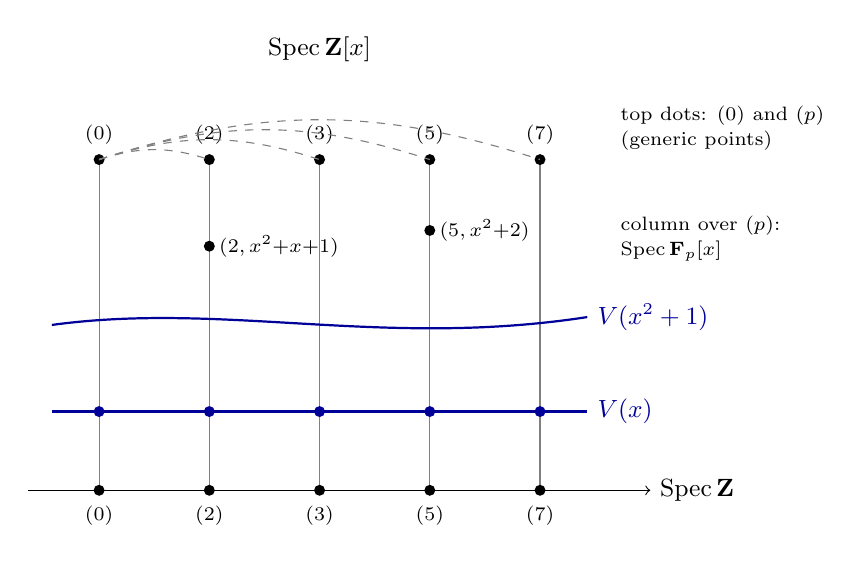
\begin{tikzpicture}[scale=1.0,every node/.style={font=\small},dot/.style={circle,fill,inner sep=1.4pt}]
\node at (3.2,5.6) {\textbf{$\Spec\Z[x]$}};
\draw[->] (-0.5,0) -- (7.4,0) node[right] {$\Spec\Z$};
\foreach \x/\l in {0.4/(0),1.8/(2),3.2/(3),4.6/(5),6.0/(7)}{
  \draw[gray] (\x,0.0) -- (\x,4.2);
  \node[dot] at (\x,0) {};
  \node[below=2pt] at (\x,0) {\scriptsize $\l$};
  \node[dot] at (\x,4.2) {};}
\node[above=2pt] at (0.4,4.2) {\scriptsize $(0)$};
\node[above=2pt] at (1.8,4.2) {\scriptsize $(2)$};
\node[above=2pt] at (3.2,4.2) {\scriptsize $(3)$};
\node[above=2pt] at (4.6,4.2) {\scriptsize $(5)$};
\node[above=2pt] at (6.0,4.2) {\scriptsize $(7)$};
\foreach \x in {1.8,3.2,4.6,6.0}{\draw[dashed,gray] (0.4,4.2) to[bend left=18] (\x,4.2);}
\node[align=left,right] at (6.9,3.2) {\scriptsize column over $(p)$:\\[-2pt]\scriptsize $\Spec\mathbf F_p[x]$};
\node[align=left,right] at (6.9,4.6) {\scriptsize top dots: $(0)$ and $(p)$\\[-2pt]\scriptsize (generic points)};
% horizontal curves
\draw[thick,blue!60!black] (-0.2,1.0) -- (6.6,1.0) node[right] {$V(x)$};
\draw[thick,blue!60!black] (-0.2,2.1) .. controls (2,2.4) and (4,1.8) .. (6.6,2.2) node[right] {$V(x^2+1)$};
\foreach \x in {0.4,1.8,3.2,4.6,6.0}{\node[dot,blue!60!black] at (\x,1.0) {};}
\node[dot] at (1.8,3.1) {}; \node[right] at (1.8,3.1) {\scriptsize $(2,x^2{+}x{+}1)$};
\node[dot] at (4.6,3.3) {}; \node[right] at (4.6,3.3) {\scriptsize $(5,x^2{+}2)$};
\end{tikzpicture}
\end{center}
\hfill$\square$

%---------------------------------------------------------------- 17
\exercise{17}{For each $f\in A$, let $X_f$ denote the complement of $V(f)$ in $X=\Spec(A)$. The sets $X_f$ are open. Show that they form a basis of open sets for the Zariski topology, and that
\begin{enumerate}[label=(\roman*),leftmargin=*]
\item $X_f\cap X_g=X_{fg}$;
\item $X_f=\emptyset\iff f$ is nilpotent;
\item $X_f=X\iff f$ is a unit;
\item $X_f=X_g\iff\rad((f))=\rad((g))$;
\item $X$ is quasi-compact (that is, every open covering of $X$ has a finite subcovering);
\item more generally, each $X_f$ is quasi-compact;
\item an open subset of $X$ is quasi-compact if and only if it is a finite union of sets $X_f$.
\end{enumerate}
The sets $X_f$ are called the \emph{basic open sets} of $X=\Spec(A)$. [To prove (v), remark that it is enough to consider a covering of $X$ by basic open sets $X_{f_i}$ $(i\in I)$. Show that the $f_i$ generate the unit ideal and hence that there is an equation of the form $1=\sum_{i\in J}g_if_i$ $(g_i\in A)$ where $J$ is some \emph{finite} subset of $I$. Then the $X_{f_i}$ $(i\in J)$ cover $X$.]}
\pf
Note $X_f=X\setminus V(f)=\{\fp:f\notin\fp\}$, and $V(f):=V(\{f\})=V((f))$.

\textbf{Basis.} Every open set is $X\setminus V(E)=X\setminus\bigcap_{f\in E}V(f)=\bigcup_{f\in E}X_f$ (15(iii)). So the $X_f$ form a basis.

(i) $\fp\notin V(f)\cup V(g)\iff f,g\notin\fp\iff fg\notin\fp$ (prime), so $X_f\cap X_g=X_{fg}$.

(ii) $X_f=\emptyset\iff f$ lies in every prime $\iff f\in\Nil$ (1.8).

(iii) $X_f=X\iff f$ lies in no prime $\iff f$ lies in no maximal ideal $\iff f$ is a unit (1.5).

(iv) $X_f=X_g\iff V(f)=V(g)\iff\rad((f))=\rad((g))$: since $\rad(\fa)=\bigcap_{\fp\in V(\fa)}\fp$ (1.14), $V(\fa)=V(\fb)$ implies $\rad\fa=\rad\fb$, and the converse is 15(i).

(v) Every open cover can be refined to a cover by basic open sets $X_{f_i}$ ($i\in I$), and a finite subcover of the refinement gives a finite subcover of the original (pick for each of finitely many $X_{f_i}$ one member of the original cover containing it). So take $X=\bigcup_{i\in I}X_{f_i}$. Then $V(\{f_i\})=\bigcap V(f_i)=\emptyset$, so the ideal generated by the $f_i$ is $(1)$ (else it lies in a maximal ideal, which is a prime in $V(\{f_i\})$). Hence $1=\sum_{i\in J}g_if_i$ with $J\subseteq I$ finite. If a prime $\fp$ were outside $\bigcup_{i\in J}X_{f_i}$, all $f_i\in\fp$ ($i\in J$), giving $1\in\fp$. So $X=\bigcup_{i\in J}X_{f_i}$.

(vi) As in (v) it suffices to consider $X_f\subseteq\bigcup_{i\in I}X_{g_i}$. Then every prime containing all $g_i$ contains $f$: $f\in\bigcap_{\fp\supseteq(g_i)}\fp=\rad((g_i:i\in I))$, so $f^n=\sum_{i\in J}h_ig_i$ for some $n$ and finite $J$. Then $X_f=X_{f^n}\subseteq\bigcup_{i\in J}X_{g_i}$: a prime $\fp$ with $f\notin\fp$ cannot contain all $g_i$, $i\in J$ (it would contain $f^n$).

(vii) ($\Leftarrow$) A finite union of quasi-compact sets is quasi-compact, and $X_f$ is quasi-compact by (vi). ($\Rightarrow$) An open $U$ is a union of basic opens; if $U$ is quasi-compact, finitely many suffice. \hfill$\square$

%---------------------------------------------------------------- 18
\exercise{18}{For psychological reasons it is sometimes convenient to denote a prime ideal of $A$ by a letter such as $x$ or $y$ when thinking of it as a point of $X=\Spec(A)$. When thinking of $x$ as a prime ideal of $A$, we denote it by $\fp_x$ (logically, of course, it is the same thing). Show that
\begin{enumerate}[label=(\roman*),leftmargin=*]
\item the set $\{x\}$ is closed (we say that $x$ is a ``closed point'') in $\Spec(A)\iff\fp_x$ is maximal;
\item $\overline{\{x\}}=V(\fp_x)$;
\item $y\in\overline{\{x\}}\iff\fp_x\subseteq\fp_y$;
\item $X$ is a $T_0$-space (this means that if $x,y$ are distinct points of $X$, then either there is a neighborhood of $x$ which does not contain $y$, or else there is a neighborhood of $y$ which does not contain $x$).
\end{enumerate}}
\pf
Write $x\leftrightarrow\fp_x$.

(ii) A closed set containing $x$ is $V(E)$ with $E\subseteq\fp_x$, hence $V(E)\supseteq V(\fp_x)$. So the smallest closed set containing $x$ is $V(\fp_x)$: $\overline{\{x\}}=V(\fp_x)$.

(i) By (ii), $\{x\}$ is closed $\iff V(\fp_x)=\{\fp_x\}\iff$ no prime strictly contains $\fp_x\iff\fp_x$ is maximal (if $\fp_x$ is not maximal it lies in a maximal ideal, a different prime; the converse is clear).

(iii) $y\in\overline{\{x\}}=V(\fp_x)\iff\fp_x\subseteq\fp_y$.

(iv) Let $x\neq y$, i.e.\ $\fp_x\neq\fp_y$. Then $\fp_x\not\subseteq\fp_y$ or $\fp_y\not\subseteq\fp_x$. In the first case $y\notin\overline{\{x\}}=V(\fp_x)$, so $X\setminus V(\fp_x)$ is an open neighbourhood of $y$ not containing $x$; in the second case symmetrically there is a neighbourhood of $x$ missing $y$. \hfill$\square$

%---------------------------------------------------------------- 19
\exercise{19}{A topological space $X$ is said to be \emph{irreducible} if $X\ne\emptyset$ and if every pair of non-empty open sets in $X$ intersect, or equivalently if every non-empty open set is dense in $X$. Show that $\Spec(A)$ is irreducible if and only if the nilradical of $A$ is a prime ideal.}
\pf
Every non-empty open set contains a non-empty basic open set, so $X$ is irreducible iff $X\neq\emptyset$ and any two non-empty basic opens meet. Now $X\ne\emptyset\iff A\ne0\iff 1\notin\Nil\iff\Nil\ne(1)$. By 17(ii), $X_f\neq\emptyset\iff f\notin\Nil$, and $X_f\cap X_g=X_{fg}$ (17(i)). So the second condition reads: $f,g\notin\Nil\Rightarrow fg\notin\Nil$, i.e.\ $\Nil$ is prime (together with $\Nil\ne(1)$). \hfill$\square$

%---------------------------------------------------------------- 20
\exercise{20}{Let $X$ be a topological space.
\begin{enumerate}[label=(\roman*),leftmargin=*]
\item If $Y$ is an irreducible (Exercise 19) subspace of $X$, then the closure $\bar Y$ of $Y$ in $X$ is irreducible.
\item Every irreducible subspace of $X$ is contained in a maximal irreducible subspace.
\item The maximal irreducible subspaces of $X$ are closed and cover $X$. They are called the \emph{irreducible components} of $X$. What are the irreducible components of a Hausdorff space?
\item If $A$ is a ring and $X=\Spec(A)$, then the irreducible components of $X$ are the closed sets $V(\fp)$, where $\fp$ is a minimal prime ideal of $A$ (Exercise 8).
\end{enumerate}}
\pf
\textbf{(i)} Let $Y$ be irreducible and $U,V$ non-empty open subsets of $\bar Y$. Pick a point of $U$; as it lies in the closure of $Y$ and $U$ is open in $\bar Y$ (so $U=\bar Y\cap U'$, $U'$ open in $X$), $U'$ meets $Y$; so $U\cap Y\ne\emptyset$, similarly $V\cap Y\ne\emptyset$. These are non-empty open subsets of $Y$, hence meet, so $U\cap V\ne\emptyset$. Also $\bar Y\ne\emptyset$.

\textbf{(ii)} Let $Y$ be irreducible and apply Zorn to the set of irreducible subspaces containing $Y$, ordered by inclusion. If $(Y_\alpha)$ is a chain, $Z=\bigcup Y_\alpha$ is irreducible: if $U,V$ are non-empty open in $Z$, choose $u\in U\cap Y_\alpha$, $v\in V\cap Y_\beta$ with (say) $Y_\alpha\subseteq Y_\beta$; then $U\cap Y_\beta,V\cap Y_\beta$ are non-empty and open in $Y_\beta$ so they meet. Hence maximal irreducible subspaces exist above every irreducible subspace.

\textbf{(iii)} If $Y$ is maximal irreducible then $\bar Y$ is irreducible by (i) and contains $Y$, so $Y=\bar Y$ is closed. Each point $\{x\}$ is irreducible, so by (ii) lies in a maximal irreducible subspace; these cover $X$.

\emph{Hausdorff spaces.} If $Y$ is irreducible with two distinct points $x,y$, take disjoint open neighbourhoods $U\ni x$, $V\ni y$ in $X$; then $U\cap Y$, $V\cap Y$ are disjoint non-empty open sets of $Y$, contradiction. So irreducible subspaces are single points: the irreducible components of a Hausdorff space are its points.

\textbf{(iv)} Let $X=\Spec A$. For a closed set $Y=V(\fa)$ put $I(Y)=\bigcap_{\fq\in Y}\fq$; then $Y=V(I(Y))$ (as $V(\fa)=V(\rad\fa)$ and $I(Y)=\rad\fa$). \emph{Claim: a closed $Y\neq\emptyset$ is irreducible $\iff I(Y)$ is prime.}
($\Rightarrow$) $I(Y)\neq(1)$. If $xy\in I(Y)$, then every $\fq\in Y$ contains $x$ or $y$, so $Y=(Y\cap V(x))\cup(Y\cap V(y))$. If both pieces were proper, their complements in $Y$ would be non-empty disjoint open subsets of $Y$, contradicting irreducibility. So $Y\subseteq V(x)$ or $V(y)$, i.e.\ $x\in I(Y)$ or $y\in I(Y)$.
($\Leftarrow$) Let $\fp=I(Y)$ be prime, so $Y=V(\fp)$. If $Y=Y_1\cup Y_2$ with $Y_i$ closed, then $\fp=I(Y_1)\cap I(Y_2)\supseteq I(Y_1)I(Y_2)$, so (primality) $\fp\supseteq I(Y_1)$, say; then $Y=V(\fp)\subseteq V(I(Y_1))=Y_1$. So $Y$ is not a union of two proper closed subsets, i.e.\ irreducible.

Hence the closed irreducible subsets are exactly the $V(\fp)$, $\fp$ prime, and $V(\fp)\subseteq V(\fq)\iff\fq\subseteq\fp$. The maximal ones are the $V(\fp)$ with $\fp$ a minimal prime. By (iii) maximal irreducible subspaces are closed, so these are exactly the irreducible components. \hfill$\square$

%---------------------------------------------------------------- 21
\exercise{21}{Let $\phi:A\to B$ be a ring homomorphism. Let $X=\Spec(A)$ and $Y=\Spec(B)$. If $\fq\in Y$, then $\phi^{-1}(\fq)$ is a prime ideal of $A$, i.e.\ a point of $X$. Hence $\phi$ induces a mapping $\phi^*:Y\to X$. Show that
\begin{enumerate}[label=(\roman*),leftmargin=*]
\item If $f\in A$ then $\phi^{*-1}(X_f)=Y_{\phi(f)}$, and hence that $\phi^*$ is continuous.
\item If $\fa$ is an ideal of $A$, then $\phi^{*-1}(V(\fa))=V(\fa^\ex)$.
\item If $\fb$ is an ideal of $B$, then $\overline{\phi^*(V(\fb))}=V(\fb^\ci)$.
\item If $\phi$ is surjective, then $\phi^*$ is a homeomorphism of $Y$ onto the closed subset $V(\Ker(\phi))$ of $X$. (In particular, $\Spec(A)$ and $\Spec(A/\Nil)$, where $\Nil$ is the nilradical of $A$, are naturally homeomorphic.)
\item If $\phi$ is injective, then $\phi^*(Y)$ is dense in $X$. More precisely, $\phi^*(Y)$ is dense in $X\iff\Ker(\phi)\subseteq\Nil$.
\item Let $\psi:B\to C$ be another ring homomorphism. Then $(\psi\circ\phi)^*=\phi^*\circ\psi^*$.
\item Let $A$ be an integral domain with just one non-zero prime ideal $\fp$, and let $K$ be the field of fractions of $A$. Let $B=(A/\fp)\times K$. Define $\phi:A\to B$ by $\phi(x)=(\bar x,x)$, where $\bar x$ is the image of $x$ in $A/\fp$. Show that $\phi^*$ is bijective but not a homeomorphism.
\end{enumerate}}
\pf
Let $Y=\Spec B$, $\phi^*(\fq)=\phi^{-1}(\fq)$.

(i) $\fq\in\phi^{*-1}(X_f)\iff f\notin\phi^{-1}(\fq)\iff\phi(f)\notin\fq\iff\fq\in Y_{\phi(f)}$. Preimages of basic opens are open, so $\phi^*$ is continuous.

(ii) $\fq\in\phi^{*-1}(V(\fa))\iff\phi^{-1}(\fq)\supseteq\fa\iff\fq\supseteq\phi(\fa)\iff\fq\supseteq\fa^\ex$.

(iii) The closure of $S\subseteq X$ is $V\bigl(\bigcap_{\fp\in S}\fp\bigr)$ (the smallest $V(E)$ containing $S$ has $E\subseteq\bigcap_S\fp$). For $S=\phi^*(V(\fb))=\{\phi^{-1}(\fq):\fq\supseteq\fb\}$:
\[
\bigcap_{\fq\supseteq\fb}\phi^{-1}(\fq)=\phi^{-1}\Bigl(\bigcap_{\fq\supseteq\fb}\fq\Bigr)=\phi^{-1}(\rad\fb)=\rad(\fb^\ci)
\]
(by 1.14 and Ex.~1.18). Hence $\overline{\phi^*(V(\fb))}=V(\rad(\fb^\ci))=V(\fb^\ci)$ by 15(i).

(iv) Let $\phi$ be surjective. $\phi^*$ maps into $V(\Ker\phi)$ since $\phi^{-1}(\fq)\supseteq\phi^{-1}(0)$. It is injective: $\phi(\phi^{-1}(\fq))=\fq$ by surjectivity, so $\phi^{-1}(\fq)=\phi^{-1}(\fq')\Rightarrow\fq=\fq'$. It is onto $V(\Ker\phi)$: if $\fp\supseteq\Ker\phi$ is prime then $\phi(\fp)$ is a prime of $B$ and $\phi^{-1}(\phi(\fp))=\fp+\Ker\phi=\fp$. It is closed: for $\fb\subseteq B$, $\phi^*(V(\fb))=V(\fb^\ci)$ (given $\fp\supseteq\fb^\ci$ then $\phi(\fp)\supseteq\phi(\phi^{-1}\fb)=\fb$ and $\phi^*(\phi(\fp))=\fp$; the other inclusion from (iii)). A continuous closed bijection onto $V(\Ker\phi)$ is a homeomorphism. For $A\to A/\Nil$ we have $V(\Nil)=X$, so $\Spec(A/\Nil)\cong\Spec A$.

(v) By (iii) with $\fb=0$: $\overline{\phi^*(Y)}=V(\Ker\phi)$. This equals $X$ iff every prime contains $\Ker\phi$ iff $\Ker\phi\subseteq\Nil$. In particular if $\phi$ is injective, $\phi^*(Y)$ is dense.

(vi) $(\psi\phi)^{-1}(\fr)=\phi^{-1}(\psi^{-1}(\fr))$, i.e.\ $(\psi\circ\phi)^*=\phi^*\circ\psi^*$.

(vii) Let $A$ be a domain with exactly one non-zero prime $\fp$, $K=\operatorname{Frac}A$, $B=(A/\fp)\times K$, $\phi(x)=(\bar x,x)$ (an injective ring homomorphism). Since $A$ has a non-zero prime it is not a field, so it has a maximal ideal, which is a non-zero prime, hence $\fp$ is maximal and $A/\fp$ is a field. Thus $B$ is a product of two fields and $\Spec B=\{\fq_1,\fq_2\}$ with $\fq_1=0\times K$, $\fq_2=(A/\fp)\times0$; both are closed points, so $\Spec B$ is discrete. We have $\phi^*(\fq_1)=\{x:\bar x=0\}=\fp$ and $\phi^*(\fq_2)=\{x:x=0\}=0$. So $\phi^*$ is a bijection onto $\Spec A=\{0,\fp\}$. In $\Spec A$ the closed sets are $\emptyset,\{\fp\}=V(\fp),X$ (the point $0$ is dense), so $\{0\}$ is open but $\{\fp\}$ is not open; yet $\{\fq_1\}$ is open in $\Spec B$ and maps to $\{\fp\}$. So $\phi^*$ is not open, hence not a homeomorphism. \hfill$\square$

%---------------------------------------------------------------- 22
\exercise{22}{Let $A=\prod_{i=1}^nA_i$ be the direct product of rings $A_i$. Show that $\Spec(A)$ is the disjoint union of open (and closed) subspaces $X_i$, where $X_i$ is canonically homeomorphic with $\Spec(A_i)$.

Conversely, let $A$ be any ring. Show that the following statements are equivalent:
\begin{enumerate}[label=(\roman*),leftmargin=*]
\item $X=\Spec(A)$ is disconnected.
\item $A\cong A_1\times A_2$ where neither of the rings $A_1,A_2$ is the zero ring.
\item $A$ contains an idempotent $\ne0,1$.
\end{enumerate}
In particular, the spectrum of a local ring is always connected (Exercise 12).}
\pf
\textbf{Part 1.} Let $A=\prod_{i=1}^nA_i$ and $e_i=(0,\dots,1,\dots,0)$. These are idempotents with $e_ie_j=0$ ($i\ne j$), $\sum e_i=1$. For a prime $\fp$: $e_i(1-e_i)=0$ so $e_i\in\fp$ or $1-e_i\in\fp$, not both. Since $e_ie_j=0\in\fp$ at most one $e_i\notin\fp$, and not all lie in $\fp$ (as $\sum e_i=1$). So $X=\bigsqcup_iX_{e_i}$ (disjoint union of open sets), hence each $X_{e_i}$ is also closed. Moreover $X_{e_i}=V(1-e_i)$ (by the above dichotomy). Let $p_i:A\to A_i$ be the projection, surjective with kernel $(1-e_i)$. By 21(iv), $\Spec A_i\to V(\Ker p_i)=V(1-e_i)=X_{e_i}$ is a homeomorphism.

\textbf{Part 2.} For a ring $A$ we show (i)$\Rightarrow$(iii)$\Rightarrow$(ii)$\Rightarrow$(i).

(i)$\Rightarrow$(iii). Let $X=V(\fa)\sqcup V(\fb)$ with both non-empty (disconnected means a disjoint union of two non-empty closed, equivalently open, sets). From $V(\fa)\cap V(\fb)=V(\fa+\fb)=\emptyset$ we get $\fa+\fb=(1)$ (else a maximal ideal contains both). From $V(\fa)\cup V(\fb)=V(\fa\fb)=X$ we get $\fa\fb\subseteq\Nil$. Write $1=x+y$ with $x\in\fa$, $y\in\fb$; then $xy\in\Nil$, say $(xy)^n=0$. Expanding $1=(x+y)^{2n}$ shows $1\in(x^n,y^n)$: write $1=e+f$, $e\in(x^n)\subseteq\fa$, $f\in(y^n)\subseteq\fb$. Then $ef\in(x^ny^n)=0$, so $e(1-e)=ef=0$: $e$ is idempotent. If $e=0$ then $1=f\in\fb$, $V(\fb)=\emptyset$, contradiction; if $e=1$ then $1\in\fa$, $V(\fa)=\emptyset$, contradiction. So $e\ne0,1$.

(iii)$\Rightarrow$(ii). For an idempotent $e\ne0,1$, the map $A\to Ae\times A(1-e)$, $x\mapsto(xe,x(1-e))$ is a ring isomorphism (injective: $xe=0=x(1-e)\Rightarrow x=0$; surjective: $ae+b(1-e)\mapsto(ae,b(1-e))$), where $Ae$ has identity $e\ne0$ and $A(1-e)$ has identity $1-e\ne0$; neither factor is the zero ring.

(ii)$\Rightarrow$(i). By Part 1, $\Spec(A_1\times A_2)=X_1\sqcup X_2$ with $X_i\cong\Spec A_i$ non-empty (since $A_i\ne0$), open and closed.

\textbf{Local rings.} A local ring has no idempotents $\neq0,1$ (Ex.~12), so (iii) fails and $\Spec A$ is connected. \hfill$\square$

%---------------------------------------------------------------- 23
\exercise{23}{Let $A$ be a Boolean ring (Exercise 11), and let $X=\Spec(A)$.
\begin{enumerate}[label=(\roman*),leftmargin=*]
\item For each $f\in A$, the set $X_f$ (Exercise 17) is both open and closed in $X$.
\item Let $f_1,\dots,f_n\in A$. Show that $X_{f_1}\cup\cdots\cup X_{f_n}=X_f$ for some $f\in A$.
\item The sets $X_f$ are the only subsets of $X$ which are both open and closed. [Let $Y\subseteq X$ be both open and closed. Since $Y$ is open, it is a union of basic open sets $X_f$. Since $Y$ is closed and $X$ is quasi-compact (Exercise 17), $Y$ is quasi-compact. Hence $Y$ is a finite union of basic open sets; now use (ii) above.]
\item $X$ is a compact Hausdorff space.
\end{enumerate}}
\pf
Let $A$ be Boolean, so $f(1-f)=0$ for all $f$.

(i) Each prime contains exactly one of $f,1-f$; so $X_f=\{\fp:f\notin\fp\}=\{\fp:1-f\in\fp\}=V(1-f)$ is closed. It is open by definition.

(ii) By Ex.~11(iii), $(f_1,\dots,f_n)=(f)$ for some $f$. Then $V(f)=V(\{f_1,\dots,f_n\})=\bigcap V(f_i)$, so $X_f=\bigcup X_{f_i}$.

(iii) Each $X_f$ is clopen. Conversely let $Y$ be clopen. As $Y$ is open it is a union of basic open sets; as $Y$ is closed in the quasi-compact space $X$ (17(v)), $Y$ is quasi-compact; hence $Y=X_{f_1}\cup\dots\cup X_{f_n}=X_f$ by (ii).

(iv) $X$ is quasi-compact (17(v)). Hausdorff: let $\fp\ne\fq$ be primes; they are maximal (Ex.~11(ii)), so $\fp\not\subseteq\fq$, and there is $f\in\fp\setminus\fq$. Then $\fq\in X_f$, and $1-f\notin\fp$ (else $1\in\fp$) so $\fp\in X_{1-f}$, and $X_f\cap X_{1-f}=X_{f(1-f)}=X_0=\emptyset$. So $X$ is compact Hausdorff. \hfill$\square$

%---------------------------------------------------------------- 24
\exercise{24}{Let $L$ be a lattice, in which the sup and inf of two elements $a,b$ are denoted by $a\vee b$ and $a\wedge b$ respectively. $L$ is a \emph{Boolean lattice} (or \emph{Boolean algebra}) if
\begin{enumerate}[label=(\roman*),leftmargin=*]
\item $L$ has a least element and a greatest element (denoted by $0$, $1$ respectively).
\item Each of $\vee,\wedge$ is distributive over the other.
\item Each $a\in L$ has a unique ``complement'' $a'\in L$ such that $a\vee a'=1$ and $a\wedge a'=0$.
\end{enumerate}
(For example, the set of all subsets of a set, ordered by inclusion, is a Boolean lattice.)

Let $L$ be a Boolean lattice. Define addition and multiplication in $L$ by the rules
\[a+b=(a\wedge b')\vee(a'\wedge b),\qquad ab=a\wedge b.\]
Verify that in this way $L$ becomes a Boolean ring, say $A(L)$.

Conversely, starting from a Boolean ring $A$, define an ordering on $A$ as follows: $a\le b$ means that $a=ab$. Show that, with respect to this ordering, $A$ is a Boolean lattice. [The sup and inf are given by $a\vee b=a+b+ab$ and $a\wedge b=ab$, and the complement by $a'=1-a$.] In this way we obtain a one-to-one correspondence between (isomorphism classes of) Boolean rings and (isomorphism classes of) Boolean lattices.}
\pf
\textbf{Lattice facts.} In a Boolean lattice $L$: $a\wedge1=a$, $a\vee0=a$, $a\wedge0=0$, $a\vee1=1$; $a''=a$ (since $a$ is a complement of $a'$ and complements are unique); and De Morgan: $(a\vee b)'=a'\wedge b'$, because $(a\vee b)\vee(a'\wedge b')=(a\vee b\vee a')\wedge(a\vee b\vee b')=1$ and $(a\vee b)\wedge a'\wedge b'=0$ (distributivity), and by uniqueness; dually $(a\wedge b)'=a'\vee b'$.

\textbf{$L\mapsto A(L)$ is a Boolean ring.} Define $a+b=(a\wedge b')\vee(a'\wedge b)$, $ab=a\wedge b$.
\begin{itemize}[leftmargin=*]
\item $+$ is commutative (the formula is symmetric); $a+0=(a\wedge1)\vee(a'\wedge0)=a$; $a+a=(a\wedge a')\vee(a'\wedge a)=0$, so $-a=a$.
\item Associativity. If $s=a+b$ then $s'=(a'\vee b)\wedge(a\vee b')=(a\wedge b)\vee(a'\wedge b')$ (De Morgan and distributivity). So
\[(a+b)+c=(s\wedge c')\vee(s'\wedge c)=(a\wedge b'\wedge c')\vee(a'\wedge b\wedge c')\vee(a'\wedge b'\wedge c)\vee(a\wedge b\wedge c),\]
which is symmetric in $a,b,c$. Hence $(a+b)+c=(b+c)+a=a+(b+c)$.
\item $\wedge$ is associative, commutative, with identity $1$.
\item Distributivity: $a(b+c)=(a\wedge b\wedge c')\vee(a\wedge b'\wedge c)$, while $ab+ac=\bigl((a\wedge b)\wedge(a'\vee c')\bigr)\vee\bigl((a'\vee b')\wedge a\wedge c\bigr)=(a\wedge b\wedge c')\vee(a\wedge b'\wedge c)$ (terms containing $a\wedge a'$ vanish).
\item $a\cdot a=a\wedge a=a$: Boolean.
\end{itemize}

\textbf{$A\mapsto L(A)$ is a Boolean lattice.} Let $A$ be Boolean (so $2x=0$) and define $a\le b\iff a=ab$.
\begin{itemize}[leftmargin=*]
\item Partial order: $a=a\cdot a$; $a=ab,b=ba\Rightarrow a=b$; $a=ab,b=bc\Rightarrow a=abc=ac$.
\item $a\wedge b=ab$: $ab\le a,b$; and $c\le a,c\le b$ give $c\cdot ab=(ca)b=cb=c$. $a\vee b=a+b+ab$: $a(a+b+ab)=a+2ab=a$, so $a\le a+b+ab$, same for $b$; if $a,b\le c$ then $(a+b+ab)c=a+b+ab$.
\item Least element $0$ ($0=0\cdot a$), greatest element $1$ ($a=a\cdot1$).
\item $a(b\vee c)=ab+ac+abc=(a\wedge b)\vee(a\wedge c)$; and $(a\vee b)\wedge(a\vee c)=(a+b+ab)(a+c+ac)=a+bc+abc=a\vee(b\wedge c)$ (collecting the nine products and using $2x=0$).
\item Complement $a'=1-a=1+a$: $a\wedge a'=a+a^2=0$, $a\vee a'=a+(1+a)+0=1$, and if $ac=0$, $a+c+ac=1$ then $c=1+a$: unique.
\end{itemize}

\textbf{The two constructions are inverse.} Starting from $A$, form $L(A)$ and then $A(L(A))$: its product is $a\wedge b=ab$, and its sum is $(a\wedge b')\vee(a'\wedge b)=x\vee y$ with $x=a(1+b)=a+ab$, $y=b+ab$; since $xy=a b+ab+ab+ab=0$, $x\vee y=x+y=a+b+2ab=a+b$. So we recover $A$. Starting from $L$, form $A(L)$ and then $L(A(L))$: $a\le b\iff a=a\wedge b$ is the original order of $L$, and $\vee,\wedge$ are determined by the order. So we recover $L$. Hence the two constructions give a bijection between isomorphism classes of Boolean rings and Boolean lattices. \hfill$\square$

%---------------------------------------------------------------- 25
\exercise{25}{From the last two exercises deduce Stone's theorem, that every Boolean lattice is isomorphic to the lattice of open-and-closed subsets of some compact Hausdorff topological space.}
\pf
Let $L$ be a Boolean lattice, $A=A(L)$ its Boolean ring (Ex.~24), $X=\Spec A$, a compact Hausdorff space (Ex.~23). By 23(i),(iii) the clopen subsets of $X$ are exactly the $X_f$, $f\in A$. Define $\theta:A\to\{\text{clopen sets}\}$, $f\mapsto X_f$; it is onto.

\emph{Injective.} If $X_f=X_g$ then $\rad((f))=\rad((g))$ (17(iv)). In a Boolean ring $g^n=g$, so $\rad(\fa)=\fa$ for every ideal $\fa$; hence $(f)=(g)$, i.e.\ $f=gu$, $g=fv$, so $fg=gug=gu=f$ and likewise $fg=g$: $f=g$.

\emph{Order.} $f\le g\iff f=fg\iff X_f=X_{fg}=X_f\cap X_g\iff X_f\subseteq X_g$ (using 17(i) and injectivity of $\theta$ for $\Leftarrow$).

A bijection preserving the order in both directions is an isomorphism of lattices (sup and inf are determined by the order). Since the order of $L$ is the order of $L(A(L))$, $L\cong$ the lattice of open-and-closed subsets of the compact Hausdorff space $X$ under $\cup,\cap$. \hfill$\square$

%---------------------------------------------------------------- 26
\exercise{26}{Let $A$ be a ring. The subspace of $\Spec(A)$ consisting of the maximal ideals of $A$, with the induced topology, is called the \emph{maximal spectrum} of $A$ and is denoted by $\Max(A)$. For arbitrary commutative rings it does not have the nice functorial properties of $\Spec(A)$ (see Exercise 21), because the inverse image of a maximal ideal under a ring homomorphism need not be maximal.

Let $X$ be a compact Hausdorff space and let $C(X)$ denote the ring of all real-valued continuous functions on $X$ (add and multiply functions by adding and multiplying their values). For each $x\in X$, let $\fm_x$ be the set of all $f\in C(X)$ such that $f(x)=0$. The ideal $\fm_x$ is maximal, because it is the kernel of the (surjective) homomorphism $C(X)\to\R$ which takes $f$ to $f(x)$. If $\tilde X$ denotes $\Max(C(X))$, we have therefore defined a mapping $\mu:X\to\tilde X$, namely $x\mapsto\fm_x$.

We shall show that $\mu$ is a homeomorphism of $X$ onto $\tilde X$.
\begin{enumerate}[label=(\roman*),leftmargin=*]
\item Let $\fm$ be any maximal ideal of $C(X)$, and let $V=V(\fm)$ be the set of common zeros of the functions in $\fm$: that is, $V=\{x\in X:f(x)=0\text{ for all }f\in\fm\}$. Suppose that $V$ is empty. Then for each $x\in X$ there exists $f_x\in\fm$ such that $f_x(x)\ne0$. Since $f_x$ is continuous, there is an open neighborhood $U_x$ of $x$ in $X$ on which $f_x$ does not vanish. By compactness a finite number of the neighborhoods, say $U_{x_1},\dots,U_{x_n}$, cover $X$. Let $f=f_{x_1}^2+\cdots+f_{x_n}^2$. Then $f$ does not vanish at any point of $X$, hence is a unit in $C(X)$. But this contradicts $f\in\fm$. Hence $V$ is not empty. Let $x$ be a point of $V$. Then $\fm\subseteq\fm_x$, hence $\fm=\fm_x$ because $\fm$ is maximal. Hence $\mu$ is surjective.
\item By Urysohn's lemma (this is the only non-trivial fact required in the argument) the continuous functions separate the points of $X$. Hence $x\ne y\Rightarrow\fm_x\ne\fm_y$, and therefore $\mu$ is injective.
\item Let $f\in C(X)$; let $U_f=\{x\in X:f(x)\ne0\}$ and let $\tilde U_f=\{\fm\in\tilde X:f\notin\fm\}$. Show that $\mu(U_f)=\tilde U_f$. The open sets $U_f$ (resp.\ $\tilde U_f$) form a basis of the topology of $X$ (resp.\ $\tilde X$) and therefore $\mu$ is a homeomorphism.
\end{enumerate}
Thus $X$ can be reconstructed from the ring of functions $C(X)$.}
\pf
Parts (i) and (ii) are proved in the text (compactness gives a point of $V(\fm)$, hence $\mu$ is surjective; Urysohn's lemma gives injectivity: for $x\ne y$ there is a continuous $f$ with $f(x)=0$, $f(y)=1$, so $f\in\fm_x\setminus\fm_y$). So $\mu:X\to\tilde X=\Max C(X)$, $x\mapsto\fm_x$, is a bijection. It remains to do (iii).

(iii) For $f\in C(X)$: $x\in U_f\iff f(x)\ne0\iff f\notin\fm_x\iff\mu(x)\in\tilde U_f$. As $\mu$ is bijective, $\mu(U_f)=\tilde U_f$.

\emph{Bases.} The $U_f$ are open (continuity). They form a basis: let $W\subseteq X$ be open and $x\in W$. $X$ is compact Hausdorff hence normal, so Urysohn's lemma gives a continuous $g:X\to[0,1]$ with $g(x)=1$ and $g=0$ on the closed set $X\setminus W$. Then $x\in U_g\subseteq W$. The $\tilde U_f=\tilde X\cap X_f$ form a basis of the subspace topology of $\tilde X\subseteq\Spec C(X)$ (the $X_f$ are a basis of $\Spec$).

Thus $\mu$ is a bijection carrying a basis of $X$ onto a basis of $\tilde X$, so $\mu$ and $\mu^{-1}$ are open maps, i.e.\ $\mu$ is a homeomorphism. \hfill$\square$

%---------------------------------------------------------------- 27
\exercise{27}{(\emph{Affine algebraic varieties.}) Let $k$ be an algebraically closed field and let $f_\alpha(t_1,\dots,t_n)=0$ be a set of polynomial equations in $n$ variables with coefficients in $k$. The set $X$ of all points $x=(x_1,\dots,x_n)\in k^n$ which satisfy these equations is an \emph{affine algebraic variety}.

Consider the set of all polynomials $g\in k[t_1,\dots,t_n]$ with the property that $g(x)=0$ for all $x\in X$. This set is an ideal $I(X)$ in the polynomial ring, and is called the \emph{ideal of the variety} $X$. The quotient ring $P(X)=k[t_1,\dots,t_n]/I(X)$ is the ring of polynomial functions on $X$, because two polynomials $g,h$ define the same polynomial function on $X$ if and only if $g-h$ vanishes at every point of $X$, that is, if and only if $g-h\in I(X)$.

Let $\xi_i$ $(1\le i\le n)$ be the image of $t_i$ in $P(X)$. The $\xi_i$ are the \emph{coordinate functions} on $X$: if $x\in X$, then $\xi_i(x)$ is the $i$th coordinate of $x$. $P(X)$ is generated as a $k$-algebra by the coordinate functions, and is called the \emph{coordinate ring} (or \emph{affine algebra}) of $X$.

As in Exercise 26, for each $x\in X$ let $\fm_x$ be the ideal of all $f\in P(X)$ such that $f(x)=0$; it is a maximal ideal of $P(X)$. Hence, if $\tilde X=\Max(P(X))$, we have defined a mapping $\mu:X\to\tilde X$, namely $x\mapsto\fm_x$. It is easy to show that $\mu$ is injective: if $x\ne y$, we must have $x_i\ne y_i$ for some $i$, and hence $\xi_i-x_i$ is in $\fm_x$ but not in $\fm_y$, so that $\fm_x\ne\fm_y$. What is less obvious (but still true) is that $\mu$ is \emph{surjective}. This is one form of Hilbert's Nullstellensatz (see Chapter 7).}
\pf
As printed, Exercise 27 sets up notation: $k=\bar k$, $X\subseteq k^n$ an affine variety, $I(X)$ its ideal, $P(X)=k[t_1,\dots,t_n]/I(X)$, and the map $\mu:X\to\tilde X=\Max P(X)$, $x\mapsto\fm_x$, and then \emph{asserts} that $\mu$ is injective and (``less obvious but still true'') surjective. There is no explicit task, but for completeness the assertions:

\emph{$\fm_x$ is maximal:} it is the kernel of the surjective evaluation $P(X)\to k$, $f\mapsto f(x)$ (surjective since $k\subseteq P(X)$).

\emph{$\mu$ injective:} if $x\neq y$ then $x_i\ne y_i$ for some $i$ and the coordinate function $\xi_i-x_i$ lies in $\fm_x\setminus\fm_y$.

\emph{$\mu$ surjective} (this is the weak Nullstellensatz): a maximal ideal $\fm\subset P(X)$ pulls back to a maximal ideal $M\subset k[t_1,\dots,t_n]$ containing $I(X)$; since $k$ is algebraically closed, $M=(t_1-a_1,\dots,t_n-a_n)$ for some $a\in k^n$. Every defining equation $f_\alpha$ of $X$ lies in $I(X)\subseteq M$, hence $f_\alpha(a)=0$, so $a\in X$ and $\fm=\fm_a$. (This uses the Nullstellensatz, proved in Chapter 7.) \hfill$\square$

%---------------------------------------------------------------- 28
\exercise{28}{Let $f_1,\dots,f_m$ be elements of $k[t_1,\dots,t_n]$. They determine a \emph{polynomial mapping} $\phi:k^n\to k^m$: if $x\in k^n$, the coordinates of $\phi(x)$ are $f_1(x),\dots,f_m(x)$.

Let $X,Y$ be affine algebraic varieties in $k^n,k^m$ respectively. A mapping $\phi:X\to Y$ is said to be \emph{regular} if $\phi$ is the restriction to $X$ of a polynomial mapping from $k^n$ to $k^m$.

If $\eta$ is a polynomial function on $Y$, then $\eta\circ\phi$ is a polynomial function on $X$. Hence $\phi$ induces a $k$-algebra homomorphism $P(Y)\to P(X)$, namely $\eta\mapsto\eta\circ\phi$. Show that in this way we obtain a one-to-one correspondence between the regular mappings $X\to Y$ and the $k$-algebra homomorphisms $P(Y)\to P(X)$.}
\pf
Let $X\subseteq k^n$, $Y\subseteq k^m$, and $\xi_1,\dots,\xi_m$ the coordinate functions on $Y$; they generate $P(Y)$ as a $k$-algebra. Given a regular map $\phi=(f_1,\dots,f_m):X\to Y$ ($f_j\in k[t_1,\dots,t_n]$), define $\phi^\sharp:P(Y)\to P(X)$, $\eta\mapsto\eta\circ\phi$. It is well defined: if $\eta=h|_Y$ with $h\in k[s_1,\dots,s_m]$, then $\eta\circ\phi=h(f_1,\dots,f_m)|_X\in P(X)$. It is clearly a $k$-algebra homomorphism. We show
\[
\Phi:\{\text{regular maps }X\to Y\}\longrightarrow\operatorname{Hom}_{k\text{-alg}}(P(Y),P(X)),\qquad\phi\mapsto\phi^\sharp
\]
is bijective.

\emph{Injective.} $\phi^\sharp(\xi_j)=\xi_j\circ\phi=\phi_j$, the $j$-th coordinate of $\phi$. If $\phi^\sharp=\psi^\sharp$ then $\phi_j=\psi_j$ as functions on $X$ for all $j$, so $\phi=\psi$.

\emph{Surjective.} Let $\theta:P(Y)\to P(X)$ be a $k$-algebra homomorphism. Choose polynomials $f_j\in k[t_1,\dots,t_n]$ whose restrictions to $X$ represent $\theta(\xi_j)$, and let $\phi=(f_1,\dots,f_m):k^n\to k^m$. We check $\phi(X)\subseteq Y$. Now $Y$ is the common zero locus of $I(Y)$ (it contains the defining equations of $Y$ and every element of $I(Y)$ vanishes on $Y$). Let $h\in I(Y)\subseteq k[s_1,\dots,s_m]$; then $h(\xi_1,\dots,\xi_m)=0$ in $P(Y)$, so applying the $k$-algebra homomorphism $\theta$:
\[
0=\theta\bigl(h(\xi_1,\dots,\xi_m)\bigr)=h\bigl(\theta(\xi_1),\dots,\theta(\xi_m)\bigr)=h(f_1,\dots,f_m)|_X .
\]
So $h(\phi(x))=0$ for all $x\in X$, $h\in I(Y)$; hence $\phi(x)\in Y$. Thus $\phi:X\to Y$ is regular, and $\phi^\sharp(\xi_j)=f_j|_X=\theta(\xi_j)$. The homomorphisms $\phi^\sharp$ and $\theta$ agree on the generators $\xi_j$ of $P(Y)$, hence are equal. \hfill$\square$


\section*{Notes}
The textbook PDF is a scan without a text layer; I read the exercise statements from page images. Where the scan was ambiguous I noted it (Ex.~1.18, the superscript in the quotient inequality; Ex.~21(v), where I proved the general equivalence $\phi^*(Y)$ dense $\iff\Ker\phi\subseteq\Nil$, which contains the injective case).

\end{document}
